\documentclass[answers, 11pt]{exam}

\usepackage[spanish]{babel}
\usepackage[shortlabels]{enumitem}
\usepackage[T1]{fontenc}
\usepackage{amsmath}
\usepackage{graphicx}
\usepackage[cache=false,outputdir=./build]{minted}
\usepackage{lmodern}
\usepackage{wrapfig}
\usepackage{xcolor, color}
\definecolor{LightGray}{gray}{0.9}

\newcommand{\materia}{Analisis de Algoritmos 2024-1}
\newcommand{\tarea}{Tarea 08: Algoritmos que involucran Gráficas\\
(DFS/BFS/TopologicalSorting)}
\newcommand{\fecha}{\today}
\newcommand{\profesor}{Profesor(a): María de Luz Gasca Soto}
\newcommand{\ayudantes}{
  Rodrigo Fernando Velázquez Cruz \\
  Teresa Becerril Torres
}
\newcommand{\alumnos}{
  Alvaro Ramírez López \textbf{N° cuenta:} 316276355
}

\decimalpoint{}
\graphicspath{{img}}
% \colorsolutionboxes
\shadedsolutions

% \definecolor{SolutionBoxColor}{rgb}{0,128,255}
% \definecolor{SolutionColor}{rgb}{0,204,255}
\definecolor{SolutionColor}{rgb}{0,128,255}

\renewcommand{\familydefault}{\sfdefault}

\extrawidth{1.56cm}
\extraheadheight[1.5in]{-0.25in}
\extrafootheight[-0.175in]{-0.375in}
\firstpageheader{
}{
  \begin{minipage}[c]{3.5cm}
    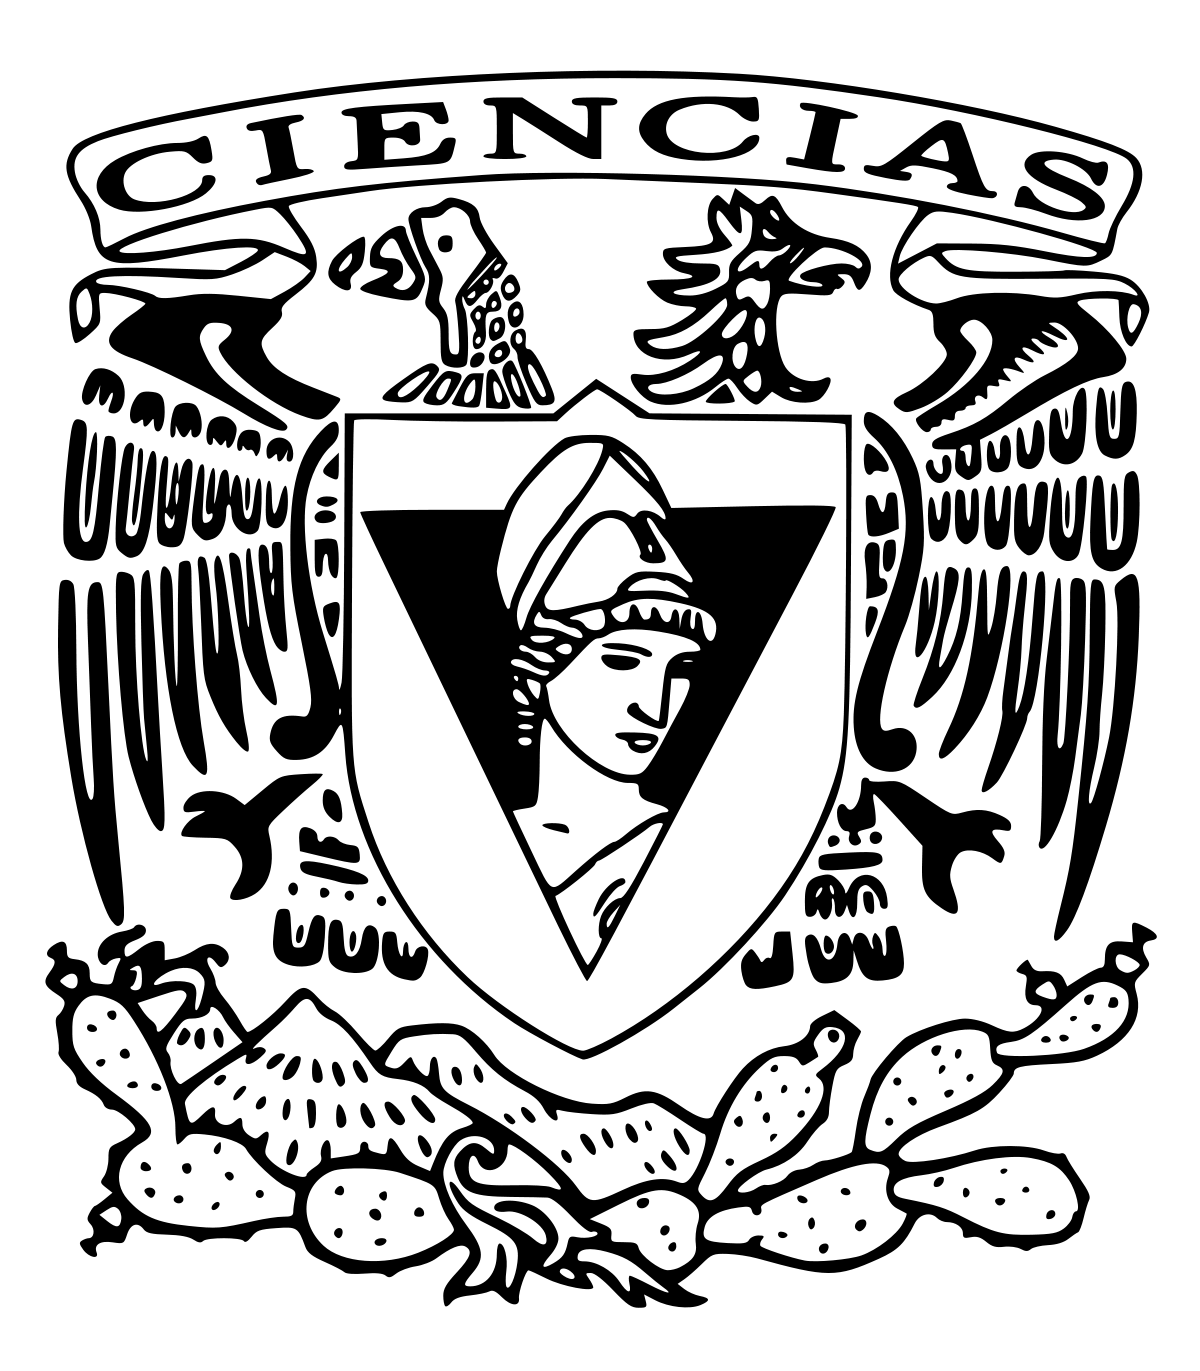
\includegraphics[width=3.5cm]{fc.png}
  \end{minipage}
  \begin{minipage}[c]{11.0cm}
    {\bfseries\huge\materia{} \\[2mm]
      \LARGE \tarea{} \\
      \large Profesor:} \profesor{} \\
    \hspace{0.1cm}
    {\bfseries\large Ayudantes:}
    \begin{minipage}[t]{8.5cm}
      \ayudantes{}\vspace{0.1cm}
    \end{minipage}\hfill\break{}
    {\bfseries\large Alumno:}
    \begin{minipage}[t]{8.5cm}
      \alumnos{}\\
    \end{minipage}\hfill\break{}
  \end{minipage}
  \begin{minipage}[c]{3.25cm}
    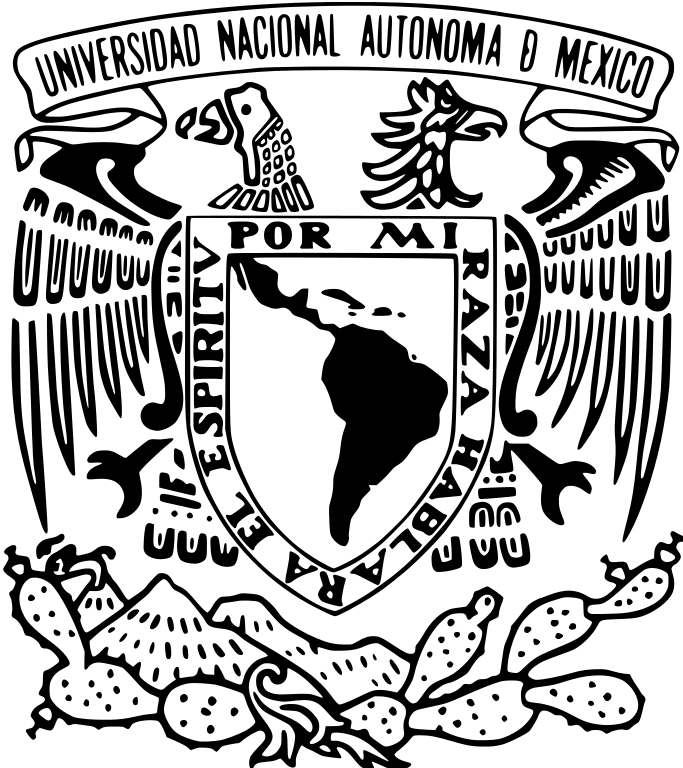
\includegraphics[width=3.25cm]{unam.png}
  \end{minipage}
}{}
\runningheader{\materia}{\tarea}{\fecha}
\runningheadrule{}
\footer{}{Página \thepage\ de \numpages}{}
\footrule{}
\renewcommand{\solutiontitle}{\noindent\textbf{Solución:}\par\noindent}



\begin{document}
\begin{questions}

  \question{El diámetro de una gráfica $G, G=(V,A)$, se define como la mayor de las longitudes de las
  rutas más cortas entre todo par de nodos en la gráfica; es decir:
  \begin{align*}
    &diam(G)= max {d(x,w) : x, w \in V(G)}
  \end{align*}
  donde $d(x,w)$ es la longitud de la ruta más corta entre los vértices $x$ y $w$.

  \textbf{Problema A:} Determinar el diámetro de un árbol
  \begin{enumerate}[a)]
    \item \textbf{Diseñar un algoritmo} de orden $O(|V|)$ que solucione el el \textbf{Problema A} y que
    presente una pareja de vértices cuya ruta más corta sea exactamente el diámetro del árbol.
    Justificar su respuesta.
    \item Presentar una gráfica \textbf{G} de al menos 17 vértices y aplicar, con detalle. el algoritmo
    diseñado en \textbf{a)}
  \end{enumerate}}

  \begin{solution}
    Aquí va la solución
  \end{solution}

  \question{Considerar los algoritmos \textbf{BFS} y \textbf{DFS}. modificar uno de ellos para que acepte como
  entrada una gráfica no conexa \textbf{D}.
  \begin{enumerate}[a)]
    \item \textbf{Resolver uno} de los siguientes problemas
      \begin{enumerate}[ ]
        \item \textbf{Problema B:} Determinar el bosque generador de una gráfica disconexa D.
        \item \textbf{Problema C:} Determinar las componentes conexas de la gráfica disconexa D.
      \end{enumerate}
    \item \textbf{Diseñe un algoritmo} que solucione el problema elegido.
    \item \textbf{Determine la complejidad del algoritmo propuesto.}
  \end{enumerate}}

  \begin{solution}
    Aquí va la solución
  \end{solution}

  \question{\textbf{Topological-Sorting (T-S)}
  \begin{enumerate}[a)]
    \item Construir una gráfica \textbf{G} de al menos 17 y 21 aristas vértices donde \textbf{sí} 
    pueda aplicarse Topological-Sorting. Aplique con detalle T-S sobre \textbf{G}.
    \item Construir una gráfica \textbf{G} de al menos 17 vértices y 23 aristas donde \textbf{no} pueda aplicarse
    Topological-Sorting, indique las razones por qué no podría aplicarse T-S
  \end{enumerate}}

  \begin{solution}
    Aquí va la solución
  \end{solution}

  \question{\textbf{Opcional} Presentar una gráfica no conexa \textbf{G}, con al menos cinco componentes conexas
  tal que G tenga al menos 24 vértices y al menos 34 aristas; aplicar, con detalle, el algoritmo
  diseñado en el Ejercicio 2.}

  \begin{solution}
    Aquí va la solución
  \end{solution}
  
\end{questions}
\end{document}